\fig{fv:f4:nonlinear}{非线性可逆磁链中，场能是电流对磁链的积分}{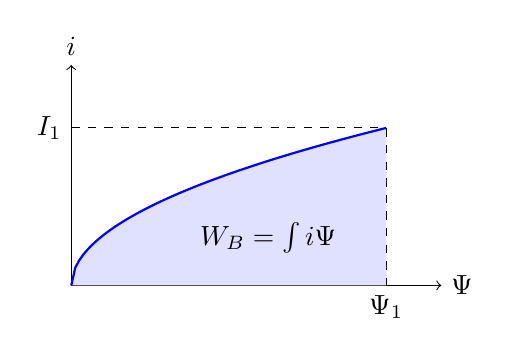
\begin{tikzpicture}[x=1cm,y=1cm]
\draw[->](0,0)--(4.7,0)node[right]{$\Psi$};\draw[->](0,0)--(0,2.8)node[above]{$i$};
\fill[blue!12](0,0)--plot[domain=0:4,samples=80](\x,{sqrt(\x)})--(4,0)--cycle;
\draw[blue,thick,domain=0:4,samples=80]plot(\x,{sqrt(\x)});\draw[dashed](0,2)--(4,2)--(4,0);
\node[below]at(4,0){$\Psi_1$};\node[left]at(0,2){$I_1$};\node at(2.5,.6){$W_B=\int i\dd\Psi$};\end{tikzpicture}}
图\ref{fv:f4:nonlinear}把磁链作为横坐标，蓝色面积才直接等于输入功。取 $i\ge0$区间内的示例 $\Psi=\alpha i^2$，反解 $i(\psi)=\alpha^{-1/2}\psi^{1/2}$，就有
\[
W_B=\alpha^{-1/2}\int_0^{\Psi_1}\psi^{1/2}\dd\psi
=\alpha^{-1/2}\left[\frac23\psi^{3/2}\right]_0^{\Psi_1}
=\frac23I_1\Psi_1,
\]并非 $I_1\Psi_1/2$。矩形剩余面积称磁共能 $W_B^*=\int_0^{I_1}\Psi(i)\dd i=I_1\Psi_1-W_B$，通常与场能不同。可逆系统有 $\dd W_B=i\dd\Psi-F\dd x$，因此 $\dd W_B^*=\Psi\dd i+F\dd x$：固定电流求力时应取 $F=\partial W_B^*/\partial x|_i$，固定磁链时取 $F=-\partial W_B/\partial x|_\Psi$。线性关系恰好把矩形分成两半，才有熟悉的二分之一系数；有磁滞时还须区分进入与返回路径，不能按单值曲线积分。
